\chapter{Plataforma de desarrollo}
\label{cap:capitulo3}

\begin{flushright}
\begin{minipage}[]{10cm}
\emph{Las herramientas adecuadas en las manos adecuadas pueden cambiar el mundo}\\
\end{minipage}\\

Steve Jobs\\
\end{flushright}

\vspace{1cm}

Tras haber establecido los objetivos que se pretenden alcanzar en este proyecto, en este capítulo se van a tratar las distintas plataformas de desarrollo tanto \textit{hardware} como \textit{software} que han contribuido para lograr dichos objetivos.

\section{Hardware}

En este apartado se van a describir el conjunto de componentes hardware que han sido necesarios adquirir para llevar a cabo este proyecto siempre primando por el menor coste de cada componente.

\subsection{Raspberry Pi 4}

La Raspberry Pi es una computadora de bajo coste y con un tamaño compacto que es ideal para proyectos de electrónica, programación y educación. Esta, en su cuarta versión, dispone de un procesador ARM Cortex-A72 de cuatro núcleos a 1,50GHz fabricado en 28nm y con 3 configuraciones de memoria. Además, entre otras características, ahora solo necesita una alimentación de USB-C, tiene 2 conectores micro HDMI, tiene conexión Wifi, Bluetooh 5.0, 2 USB 2.0 y 2 USB 3.0. Esta versión de \textit{Raspberry} permite la compatibilidad con la mayoría de accesorios gracias al conector GPIO de 40 pines y el conector \ac{CSI}. Gracias a esos 40 pines, el usuario puede interactuar con una amplia variedad de dispositivos externos como sensores, LEDs y motores, lo que lo hace excelente para proyectos de automatización y robótica. 

 Sin embargo, la \textit{Raspberry Pi} usa procesadores ARM, que, aunque eficientes energéticamente, no están optimizados para realizar tareas intensivas de \ac{IA} como entrenar modelos de redes neuronales o ejecutar inferencias en tiempo real a gran escala. En la figura \ref{fig:raspberry} se puede ver una imagen de la placa con referencia a las distintas partes de la misma. Esta pieza fue prestada por la universidad pero tiene un coste de unos 65€. 


\begin{figure} [h!]
	\begin{center}
		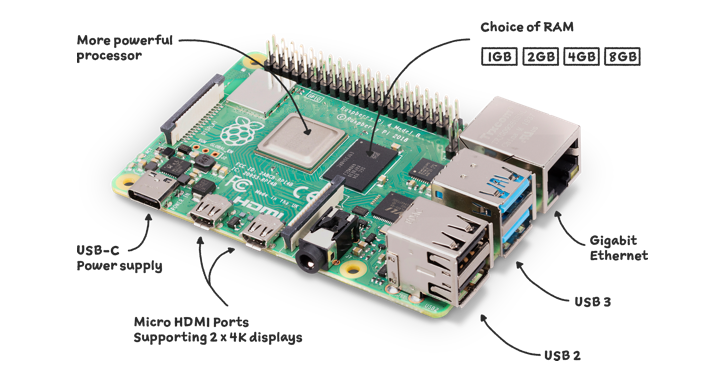
\includegraphics[width=14cm]{figs/raspberrypi4.png}
	\end{center}
	\caption{Raspberry Pi 4$^{\ref{note:enlace33}}$} 
\label{fig:raspberry}
\end{figure}\

\setcounter{footnote}{33} % Establecer la numeración de la siguiente nota al pie
\footnotetext[\value{footnote}]{\url{https://www.raspberrypi.com/products/raspberry-pi-4-model-b/}\label{note:enlace33}}

\subsection{Raspberry Pi cámara}

Esta placa que tiene un tamaño de  23.86 x 25 x 9mm (Figura \ref{fig:raspberrycam}), utiliza el sensor de imagen IMX219PQ de Sony que ofrece imágenes de vídeo de alta velocidad y alta sensibilidad. Dispone también de funciones de control automático como el control de exposición, el balance de blancos y la detección de luminancia. Esta cámara usa un cable plano que se conecta directamente al puerto \ac{CSI}.

Es muy importante destacar su bajo coste, lo que le convierte en muy buena opción para hacer aplicaciones \textit{low-cost}. Sin embargo, el cable de la cámara es bastante sensible a tensiones y torsiones y es debido a ello que aunque la cámara fue prestada por la universidad, fue necesario adquirir una unidad más a través de Amazon con un coste aproximado de 18€.    


\begin{figure} [h!]
	\begin{center}
		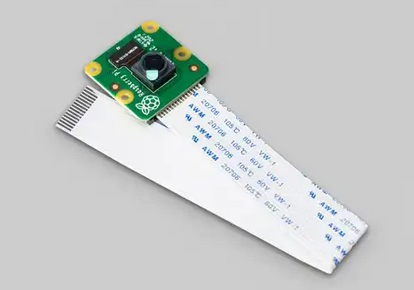
\includegraphics[width=6cm]{figs/campi.png}
	\end{center}
	\caption{Raspberry Pi Cámara V2$^{\ref{note:enlace34}}$} 
\label{fig:raspberrycam}
\end{figure}\

\setcounter{footnote}{34} % Establecer la numeración de la siguiente nota al pie
\footnotetext[\value{footnote}]{\url{https://www.raspberrypi.com/products/camera-module-v2/}\label{note:enlace34}}

\subsection{GPS NEO 6M}

Para poder identificar dónde se encuentra cada bache es necesario hacer uso de un posicionamiento global mediante satélites. En este caso se decidió comprar el módulo NEO 6M (Figura \ref{fig:gps}) cuyo asequible precio en Amazon es de 9€. El módulo utiliza el chipset u-blox NEO-6M, que proporciona un seguimiento preciso de la posición utilizando satélites \acs{GPS}, permitiendo determinar la latitud, longitud, altitud, y velocidad.Además, incluye una antena cerámica externa de alta ganancia (puede ser interna en algunas versiones), que mejora la recepción de la señal \acs{GPS}, incluso en áreas con una señal débil.

Tiene una precisión de aproximadamente 2.5 metros en condiciones abiertas. Soporta hasta 22 satélites simultáneamente, lo que le permite ofrecer posicionamiento confiable y estable. Asimismo, utiliza comunicación por \ac{UART} comunmente a 9600 bps, lo que facilita su integración con muchas placas del mercado.

\begin{figure} [h!]
	\begin{center}
		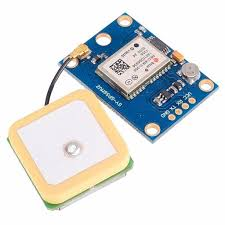
\includegraphics[width=4cm]{figs/GPSNEO6MV2.jpeg}
	\end{center}
	\caption{Módulo GPS NEO 6M$^{\ref{note:enlace35}}$} 
\label{fig:gps}
\end{figure}\

\setcounter{footnote}{35} % Establecer la numeración de la siguiente nota al pie
\footnotetext[\value{footnote}]{\url{https://www.amazon.es/dp/B088LR3488?ref}\label{note:enlace35}}


\subsection{Sevomotor Estándar Parallax}
Este tipo de servo tiene un rango de rotación de 0 a 180 grados y es compatible su control usando \ac{PWM} con un pulso alto de 0.75–2.25 ms en intervalos de 20 ms (Figura \ref{fig:parallax} izquierda). Estos tipos de servos son muy comunes para utilizar en aplicaciones de animatrónica y robótica. Sin embargo, su coste ha subido en los últimos años y el precio por unidad ronda los 17€. La universidad ha sido quien me ha prestado estos servomotores pero para esta aplicación no es necesario usarlos y se pueden sustituir por otros de menor precio que cumplan con el requisito de tener rotaciones de 0 a 180 grados (Figura \ref{fig:parallax} derecha), cuyo precio de 2 servomotores es de casi 8€. 


\begin{figure}[ht!]
	\centering
	\begin{minipage}{0.2\linewidth}
		\centering
		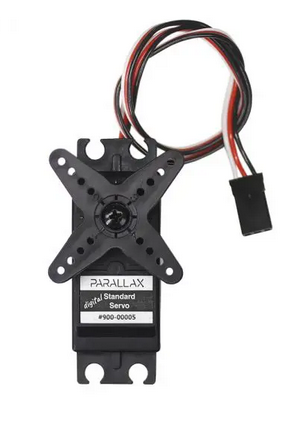
\includegraphics[width=\linewidth]{figs/parallax.png}
		\caption*{\centering Parallax $^{\ref{note:enlace36}}$} %\cite{memnon_image}
	\end{minipage}
	\hspace{2cm}
	% aquí incluir iamgen de Guerrero de terracota
	\begin{minipage}{0.33\linewidth}
		\centering
		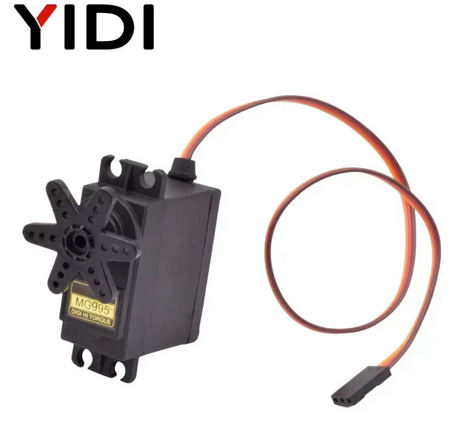
\includegraphics[width=\linewidth]{figs/diyi.png}
		\caption*{\centering YIDI $^{\ref{note:enlace37}}$} %\cite{gomezguerreros}
	\end{minipage}
	\caption{Tipos de Servomotores}
	\label{fig:parallax}
\end{figure}


\setcounter{footnote}{36} % Reiniciar la numeración de notas al pie
\footnotetext[\value{footnote}]{\url{https://www.parallax.com/product/parallax-standard-servo/}\label{note:enlace36}}

\setcounter{footnote}{37} % Reiniciar la numeración de notas al pie
\footnotetext[\value{footnote}]{\url{https://es.aliexpress.com/item/1005004551539283.html?spm=a2g0o.productlist.main.15.bee4rd8Srd8SSO&algo_pvid}\label{note:enlace37}}


\subsection{Ruedas ActivityBot}

Para implementar las ruedas de este robot, se decidió tomar las ruedas del kit robótico ActivityBot que usan este tipo de ruedas. Se trata de una rueda de plástico con neumático tipo junta tórica (Figura \ref{fig:wheel}). El perfil estrecho convierte a esta rueda en ideal para aplicaciones que requieren una dirección precisa y el diámetro de la rueda es de 66mm. La universidad ha sido quien me ha prestado su uso pero también se pueden adquirir individualmente con un coste de 4,54€ la unidad.

\begin{figure} [h!]
	\begin{center}
		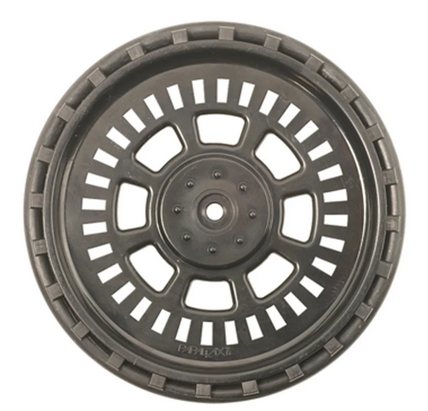
\includegraphics[width=4cm]{figs/wheel.png}
	\end{center}
	\caption{Rueda ActivityBot$^{\ref{note:enlace38}}$} 
\label{fig:wheel}
\end{figure}\

\setcounter{footnote}{38} % Establecer la numeración de la siguiente nota al pie
\footnotetext[\value{footnote}]{\url{https://es.rs-online.com/web/p/accesorios-para-kits-de-desarrollo/8430897?srsltid=AfmBOorv3a6_tQNdqAoKx_21Mn1m2MAum68oApyvr5mq8ExPTuh_CVNy}\label{note:enlace38}}

\subsection{Google Coral USB}

El \textit{Google Coral USB Accelerator} (Figura \ref{fig:googlecoral}) es un dispositivo que permite acelerar tareas de \ac{IA} en dispositivos que no cuentan con hardware especializado para ello. Está diseñado para ejecutarse con modelos de aprendizaje automático utilizando la unidad de procesamiento de tensores de Google, lo que mejora significativamente la velocidad de inferencia en aplicaciones de \acs{IA}. Está optimizado para ejecutar modelos preentrenados en \textit{TensorFlow Lite}, la versión ligera de TensorFlow diseñado para dispositivos con recursos limitados. Sólo es compatible con  las versiones desde Python 3.6 hasta la versión 3.9.

Gracias a todas esas características y para mejorar la detección de baches en tiempo real y solventar las limitaciones de la \textit{Raspberry Pi}, se ha decidido incluir este componente en el proyecto. Su precio es elevado pero se puede conseguir desde 65€.
 
\begin{figure} [h!]
	\begin{center}
		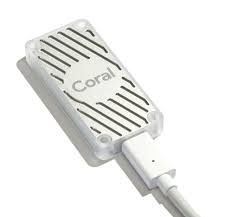
\includegraphics[width=4cm]{figs/googlecoral.png}
	\end{center}
	\caption{Google Coral USB$^{\ref{note:enlace39}}$} 
	\label{fig:googlecoral}
\end{figure}\

\setcounter{footnote}{39} % Establecer la numeración de la siguiente nota al pie
\footnotetext[\value{footnote}]{\url{https://coral.ai/products/accelerator/}\label{note:enlace39}}

\subsection{Power Bank}

Para poder alimentar a todos los componentes se ha decidido incluir en el proyecto una \textit{power bank} de bastante capacidad para que permita la autonomía del robot durante mucho tiempo. Para ello se ha elegido la \textit{Xiaomi Redmi Power Bank} de 20000 mAh cuyas dimensiones son: 73,6 x 27,3 x 154 mm. Cuando la adquirí costaba en torno a unos 20€ pero ahora se puede encontrar hasta por el doble de precio. 

\begin{figure} [h!]
	\begin{center}
		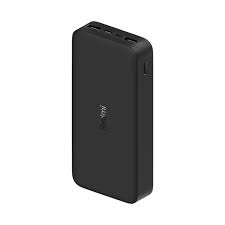
\includegraphics[width=5cm]{figs/powerbank.png}
	\end{center}
	\caption{Xiaomi Powerbank$^{\ref{note:enlace40}}$} 
	\label{fig:powerbank}
\end{figure}\

\setcounter{footnote}{40} % Establecer la numeración de la siguiente nota al pie
\footnotetext[\value{footnote}]{\url{https://buy.mi.com/es/item/3202200053}\label{note:enlace40}}

\subsection{Rueda Loca}

Para poder conseguir un movimiento correcto y poder encontrar el punto de apoyo para el robot, es necesario incluir al robot una rueda loca. Tras investigar para encontrar la que mejor encaja, se ha decidido incluir una rueda loca como la que aparece en la Figura \ref{fig:ruedaloca} que tiene las siguientes dimensiones: 5,3 x 2,9 x 2 cm. El precio de una de ellas sale por 1,13€.

\begin{figure} [h!]
	\begin{center}
		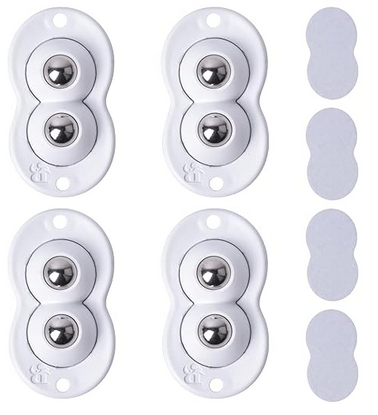
\includegraphics[width=4cm]{figs/ruedaloca.png}
	\end{center}
	\caption{Rueda loca$^{\ref{note:enlace41}}$} 
	\label{fig:ruedaloca}
\end{figure}\

\setcounter{footnote}{41} % Establecer la numeración de la siguiente nota al pie
\footnotetext[\value{footnote}]{\url{https://www.amazon.es/dp/B0BZZCJJT8?ref=cm_sw_r_mwn_dp_N64JV6SGENWN4YPSD849&ref_=cm_sw_r_mwn_dp_N64JV6SGENWN4YPSD849&social_share=cm_sw_r_mwn_dp_N64JV6SGENWN4YPSD849&language=es-ES}\label{note:enlace41}}

\subsection{Ordenador principal}

Para poder desarrollar programas, hacer pruebas en simulación, permitir conectarse por SSH a la \textit{Raspberry Pi} y poder comandar acciones al robot; ha sido necesario tener un ordenador principal que permita realizar todas las tareas. El ordenador que aparece en la Figura \ref{fig:ordenador} es el que se ha empleado en este proyecto y cumple las características descritas en el Cuadro \ref{cuadro:carac_ordena}.


\begin{figure} [h!]
	\begin{center}
		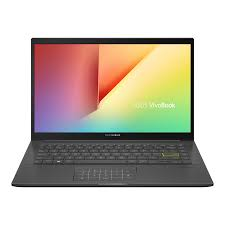
\includegraphics[width=4cm]{figs/ordenador.png}
	\end{center}
	\caption{ASUS VivoBook 14$^{\ref{note:enlace42}}$} 
	\label{fig:ordenador}
\end{figure}\

\setcounter{footnote}{42} % Establecer la numeración de la siguiente nota al pie
\footnotetext[\value{footnote}]{\url{https://www.asus.com/es/laptops/for-home/vivobook/vivobook-14-k413/}\label{note:enlace42}}

\begin{table}[H]
	\begin{center}
		\begin{tabular}{|c|c|}
			\hline
			\textbf{Características} & \textbf{Descripción} \\
			\hline
			Pantalla & 14 pulgadas, Full HD (1920x1080), tecnología LED, antirreflejo \\
			Procesador (CPU) & Intel Core i7 de 10ª generación \\
			Memoria RAM & 8GB \\
			Almacenamiento & 512GB \\
			Tarjeta gráfica (GPU) & Intel UHD Graphics de la serie Comet Lake-U GT2 \\
			Sistema Operativo & Windows 10 y Ubuntu 22.04 \\
			Puertos 1 & 1x USB 3.2 Gen 1 Tipo-A, 1x USB 3.2 Gen 1 Tipo-C, 2x USB 2.0\\  
			Puertos 2 & 1x HDMI, lector de tarjetas microSD, entrada combo de audio \\
			Conectividad & 	Wi-Fi 5 (802.11ac), Bluetooth 4.1 / 5.0 \\
			Batería & 37 Whr \\
			Peso & 1.4 kg \\
			Dimensiones & 32.5 x 21.6 x 1.99 cm \\
			\hline
		\end{tabular}
		\caption{Especificaciones técnicas del ordenador usado}
		\label{cuadro:carac_ordena}
	\end{center}
\end{table}



\section{Software}

\subsection{Freecad}

\begin{figure} [h!]
	\begin{center}
		
\includegraphics[width=4cm]{figs/freecad.png}
	\end{center}
	\caption{Logo de Freecad $^{\ref{note:enlace43}}$} 
	\label{fig:freecad}
\end{figure}\

\setcounter{footnote}{43} % Establecer la numeración de la siguiente nota al pie
\footnotetext[\value{footnote}]{\url{https://www.freecad.org/}\label{note:enlace43}}

\subsection{Python}

\begin{figure} [h!]
	\begin{center}
		
\includegraphics[width=4cm]{figs/python.png}
	\end{center}
	\caption{Logo de Python $^{\ref{note:enlace44}}$} 
	\label{fig:python}
\end{figure}\

\setcounter{footnote}{44} % Establecer la numeración de la siguiente nota al pie
\footnotetext[\value{footnote}]{\url{https://es.python.org/}\label{note:enlace44}}

\subsection{OpenCV}

\begin{figure} [h!]
	\begin{center}
		
\includegraphics[width=4cm]{figs/opencv.png}
	\end{center}
	\caption{Logo de OpenCV $^{\ref{note:enlace45}}$} 
	\label{fig:opencv}
\end{figure}\

\setcounter{footnote}{45} % Establecer la numeración de la siguiente nota al pie
\footnotetext[\value{footnote}]{\url{https://opencv.org/}\label{note:enlace45}}

\subsection{Software matemático}

numpy

\subsection{Software localización}
pynmea

\subsection{Ubuntu}

\begin{figure} [h!]
	\begin{center}
		
\includegraphics[width=4cm]{figs/ubuntu.png}
	\end{center}
	\caption{Logo de Ubuntu $^{\ref{note:enlace46}}$} 
	\label{fig:ubuntu}
\end{figure}\

\setcounter{footnote}{46} % Establecer la numeración de la siguiente nota al pie
\footnotetext[\value{footnote}]{\url{https://ubuntu.com/}\label{note:enlace46}}

\subsubsection{Ubuntu 22.04}

\subsubsection{Ubuntu 20.04}


\subsection{ROS2}


\subsubsection{ROS2 Humble}

\subsubsection{ROS2 Foxy}


\begin{figure}[ht!]
	\centering
	\begin{minipage}{0.4\linewidth}
		\centering
		
\includegraphics[width=\linewidth]{figs/foxy.png}
		\caption*{\centering Ros2 Foxy $^{\ref{note:enlace47}}$} %\cite{memnon_image}
	\end{minipage}
	\hspace{2cm}
	% aquí incluir iamgen de Guerrero de terracota
	\begin{minipage}{0.35\linewidth}
		\centering
		
\includegraphics[width=\linewidth]{figs/humble.png}
		\caption*{\centering Logo Ros2 Humble $^{\ref{note:enlace48}}$} %\cite{gomezguerreros}
	\end{minipage}
	\caption{Distribuciones de ROS2 usadas}
	\label{fig:rosdis}
\end{figure}


% Definir la primera nota al pie con el número 1
\setcounter{footnote}{47} % Reiniciar la numeración de notas al pie
\footnotetext[\value{footnote}]{\url{https://docs.ros.org/en/foxy/Installation.html}\label{note:enlace47}}

\setcounter{footnote}{48} % Reiniciar la numeración de notas al pie
\footnotetext[\value{footnote}]{\url{https://docs.ros.org/en/humble/index.html}\label{note:enlace48}}


(condensar en herramientas de simulación?? añadir xml?? sdf...)
\subsection{Ros2 Control}

\subsection{Gazebo}


\begin{figure} [h!]
	\begin{center}
		
\includegraphics[width=4cm]{figs/gazebo.png}
	\end{center}
	\caption{Logo de Gazebo $^{\ref{note:enlace49}}$} 
	\label{fig:gazebo}
\end{figure}\

\setcounter{footnote}{49} % Establecer la numeración de la siguiente nota al pie
\footnotetext[\value{footnote}]{\url{https://gazebosim.org/home}\label{note:enlace49}}

\subsection{Herramientas de visualización}

rqtimage view

Rviz
ros2 topic echo...

\begin{figure} [h!]
	\begin{center}
		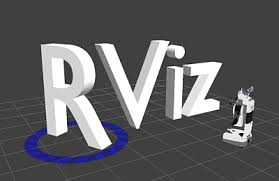
\includegraphics[width=4cm]{figs/rviz.png}
	\end{center}
	\caption{Logo de Rviz $^{\ref{note:enlace50}}$} 
	\label{fig:rviz}
\end{figure}\

\setcounter{footnote}{50} % Establecer la numeración de la siguiente nota al pie
\footnotetext[\value{footnote}]{\url{http://wiki.ros.org/rviz}\label{note:enlace50}}

\subsection{Google Colab/Jupyter Notebook}

\begin{figure} [h!]
	\begin{center}
		
\includegraphics[width=4cm]{figs/googlecolab.png}
	\end{center}
	\caption{Logo de Google Colab $^{\ref{note:enlace51}}$} 
	\label{fig:googlecolab}
\end{figure}\

\setcounter{footnote}{51} % Establecer la numeración de la siguiente nota al pie
\footnotetext[\value{footnote}]{\url{https://colab.research.google.com/}\label{note:enlace51}}

\subsection{YOLOv8}


\begin{figure} [h!]
	\begin{center}
		
\includegraphics[width=4cm]{figs/yolov8.png}
	\end{center}
	\caption{Logo de YOLOv8 $^{\ref{note:enlace52}}$} 
	\label{fig:yolov8}
\end{figure}\

\setcounter{footnote}{52} % Establecer la numeración de la siguiente nota al pie
\footnotetext[\value{footnote}]{\url{https://docs.ultralytics.com/es}\label{note:enlace52}}


\subsection{TensorFlow Lite Edge TPU}

\begin{figure} [h!]
	\begin{center}
		
\includegraphics[width=6cm]{figs/tflite.png}
	\end{center}
	\caption{Logo de TensorFlow Lite $^{\ref{note:enlace53}}$} 
	\label{fig:tflite}
\end{figure}\

\setcounter{footnote}{53} % Establecer la numeración de la siguiente nota al pie
\footnotetext[\value{footnote}]{\url{https://ai.google.dev/edge/litert}\label{note:enlace53}}


\subsection{Interfaz Web}

\subsubsection{ROS2 bridge suite}

\subsubsection{Open Street Maps}


\begin{figure} [h!]
	\begin{center}
		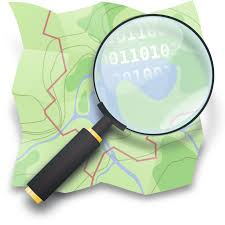
\includegraphics[width=4cm]{figs/osm.png}
	\end{center}
	\caption{Logo de Open Street Maps $^{\ref{note:enlace54}}$} 
	\label{fig:osm}
\end{figure}\

\setcounter{footnote}{54} % Establecer la numeración de la siguiente nota al pie
\footnotetext[\value{footnote}]{\url{https://www.openstreetmap.org}\label{note:enlace54}}


Mirar si hay que añadir alguna otra subsubsección
El presente proyecto trata ....\\


Después de aquí pasar al aparatado del estado del arte \\\\

En los textos puedes poner palabras en \textit{cursiva}, para aquellas expresiones en sentido \textit{figurado}, palabras como \textit{robota}, que está fuera del diccionario castellano, o bien para resaltar palabras de una colección: \textit{(a)} es la primera letra del abecedario, \textit{(b)} es la segunda, etc.\\

Al poner las dos líneas del anterior párrafo, este aparecerá separado del anterior. Si no las pongo, los párrafos aparecerán pegados. Sigue el criterio que consideres más oportuno.

\section{Segunda sección}
\label{sec:segundaseccion}

No olvides incluir imágenes y referenciarlas, como la Figura \ref{fig:roomba}.

\begin{figure} [h!]
	\begin{center}
		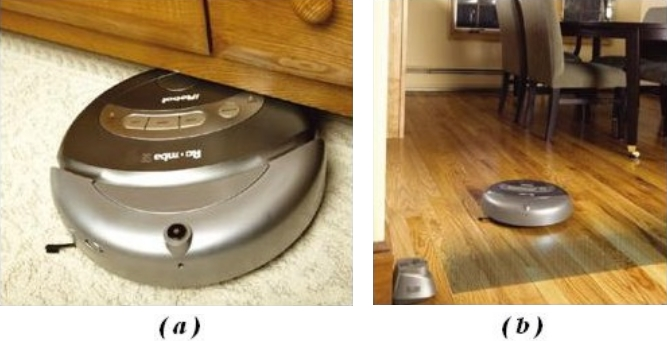
\includegraphics[width=8cm]{figs/roomba}
	\end{center}
	\caption{Robot aspirador Roomba de iRobot.}
	\label{fig:roomba}
\end{figure}\

Ni tampoco olvides de poner las URLs como notas al pie. Por ejemplo, si hablo de la Robocup\footnote{\url{http://www.robocup.org}}.

\subsection{Números}
\label{sec:subseccion}

En lugar de tener secciones interminables, como la Sección \ref{sec:robotica}, divídelas en subsecciones.

Para hablar de números, mételos en el entorno \textit{math} de \LaTeX, por ejemplo, $1.5Kg$. También puedes usar el símbolo del Euro como aquí: 1.500\euro.

\subsection{Listas}

Cuando describas una colección, usa \texttt{itemize} para ítems o \texttt{enumerate} para enumerados. Por ejemplo:

\begin{itemize}
	\item \textit{Entorno de simulación.} Hemos usado dos entornos de simulación: uno en 3D y otro en 2D.
	\item \textit{Entornos reales.} Dentro del campus, hemos realizado experimentos en Biblioteca y en el edificio de Gestión.
\end{itemize}\

\begin{enumerate}
	\item Primer elemento de la colección.
	\item Segundo elemento de la colección.
\end{enumerate}\

\paragraph{Referencias bibliográficas}
\label{sec:referencias}

Cita, sobre todo en este capítulo, referencias bibliográficas que respalden tu argumento. Para citarlas basta con poner la instrucción \verb|\cite| con el identificador de la cita. Por ejemplo: libros como \cite{vega12e}, artículos como \cite{vega19b}, URLs como \cite{vega19a}, tesis como \cite{vega18b}, congresos como \cite{vega18a}, u otros trabajos fin de grado como \cite{vega08b}.

Las referencias, con todo su contenido, están recogidas en el fichero \texttt{bibliografia.bib}. El contenido de estas referencias está en formato \texttt{BibTex}. Este formato se puede obtener en muchas ocasiones directamente, desde plataformas como \texttt{Google Scholar} u otros repositorios de recursos científicos.

Existen numerosos estilos para reflejar una referencia bibliográfica. El estilo establecido por defecto en este documento es APA, que es uno de los estilos más comunes, pero lo puedes modificar en el archivo \texttt{memoria.tex}; concretamente, cambiando el campo \verb|apalike| a otro en la instrucción \verb|\bibliographystyle{apalike}|. 

\

\

\

Y, para terminar este capítulo, resume brevemente qué vas a contar en los siguientes.
